\section{Bluetooth Low Energy}
\begin{frame}

\begin{minipage}[t]{0.45\linewidth}
\begin{figure}
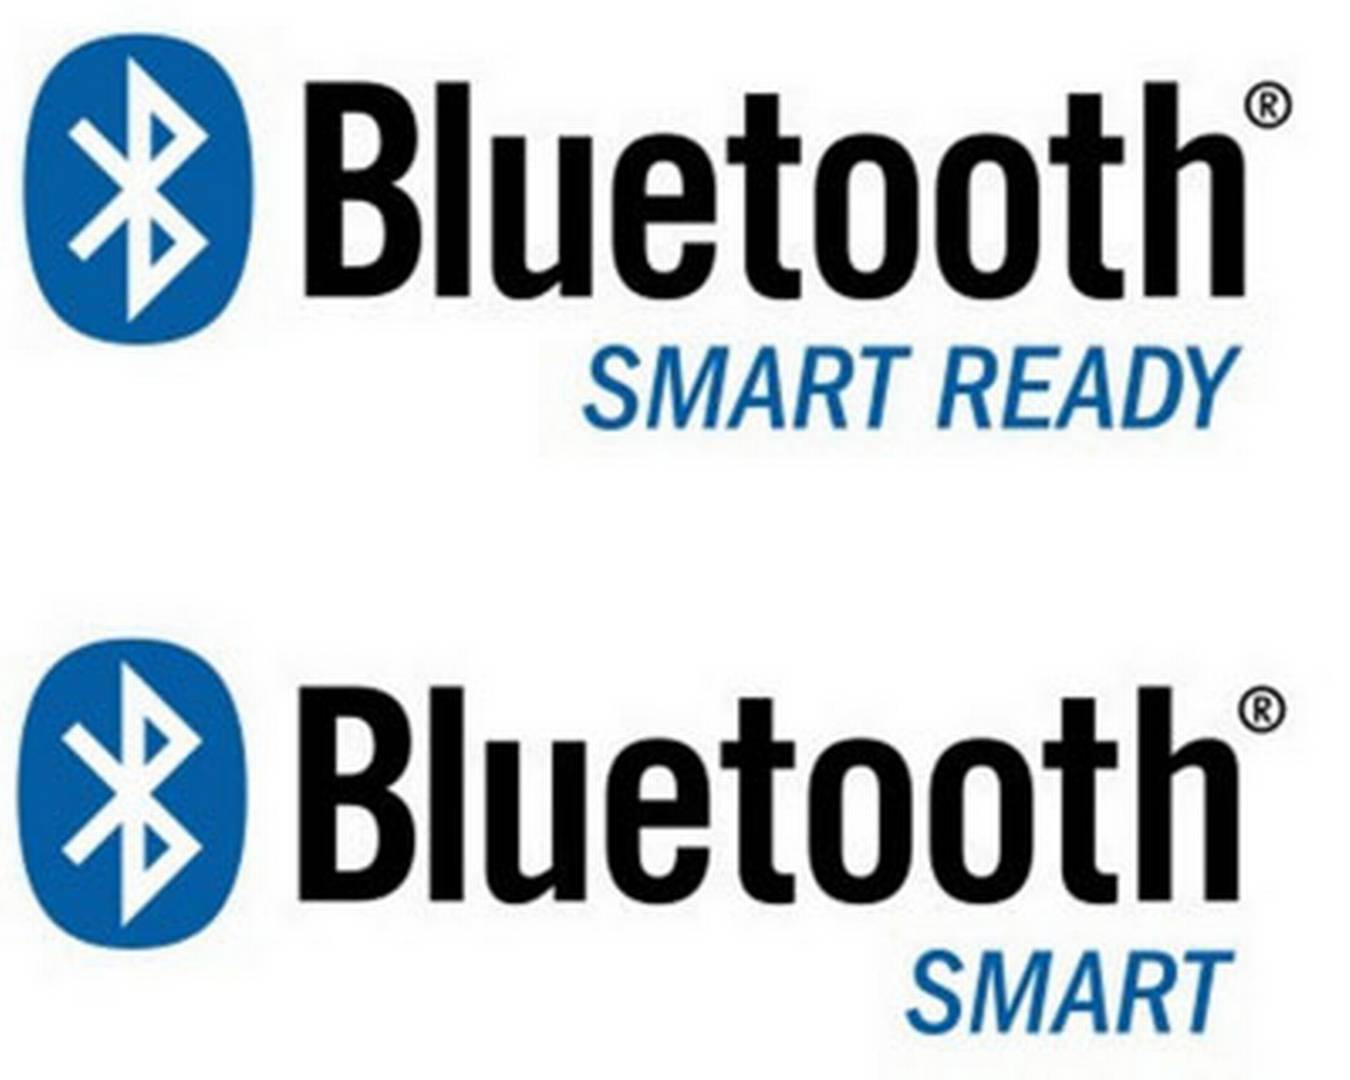
\includegraphics[height=3.25cm]{bt_logo_smart_and_ready.jpg}
\caption{Logos Bluetooth Low Energy}
\end{figure}

\end{minipage}
\begin{minipage}[t]{0.52\linewidth}
\begin{block}{Bluetooth Smart}
\begin{itemize}
\item 2006 : Wibree ( Nokia )
\item 2010 : Bluetooth 4.0
\end{itemize}
\end{block}
\begin{block}{Caractéristiques}
\begin{itemize}
\item 2.4 GHz
\item 40 cannaux
\item 1 Mbit/s
\item Conso entre 0.01W et 0.5W
\end{itemize}
\end{block}
\end{minipage}
\end{frame}

\subsection{Architecture logique}
\begin{frame}

\begin{minipage}[t]{0.45\linewidth}
graph
\end{minipage}
\begin{minipage}[t]{0.45\linewidth}
	\begin{block}{Link Layer}
		\begin{itemize}
			\item Advertising
			\item Scanning
			\item Connected
		\end{itemize}
	\end{block}
	\begin{block}{Sécurité}
		\begin{itemize}
			\item Clé côté Host
			\item AES 128
			\item Adresses :
			\begin{itemize}
				\item Publique
				\item Aléatoire
			\end{itemize}
		\end{itemize}
	\end{block}
\end{minipage}
% ici schema diff BT/BLE de bt.org
\end{frame}

\subsection{Attributs}
\begin{frame}
Attributs, profiles, services, caracteristiques
\end{frame}


